\documentclass[tikz,border=8pt]{standalone}
% Shared look for every TikZ diagram. Load with \input{../../tools/tikz-style.tex}
\usepackage[T1]{fontenc}
\usepackage{lmodern}
\renewcommand{\sfdefault}{lmr}  % diagrams use the same serif as the text
\usetikzlibrary{arrows.meta, positioning, shapes.geometric, calc, fit, backgrounds}
\definecolor{cblue}{HTML}{4C78A8}
\definecolor{corange}{HTML}{F58518}
\definecolor{cgreen}{HTML}{54A24B}
\definecolor{cred}{HTML}{E45756}
\definecolor{cpurple}{HTML}{B279A2}
\definecolor{cgrey}{HTML}{6B6B6B}
\tikzset{
  every picture/.style={font=\sffamily, line width=1.2pt},
  box/.style={draw=#1, fill=#1!12, rounded corners=4pt, align=center, inner sep=7pt, minimum height=1.1cm},
  box/.default=cgrey,
  arrow/.style={-{Stealth[length=3mm]}, draw=cgrey, line width=1.4pt},
  title/.style={font=\sffamily\bfseries\Large},
  note/.style={font=\sffamily\small, text=cgrey, align=center},
}
\AtBeginDocument{\hyphenpenalty=10000 \exhyphenpenalty=10000}

% f(x) = x^2 + exp(x^2) as a computation graph. Forward (grey): compute values. Backward (red): multiply local derivatives from f back to x; paths that meet are added.
\begin{document}
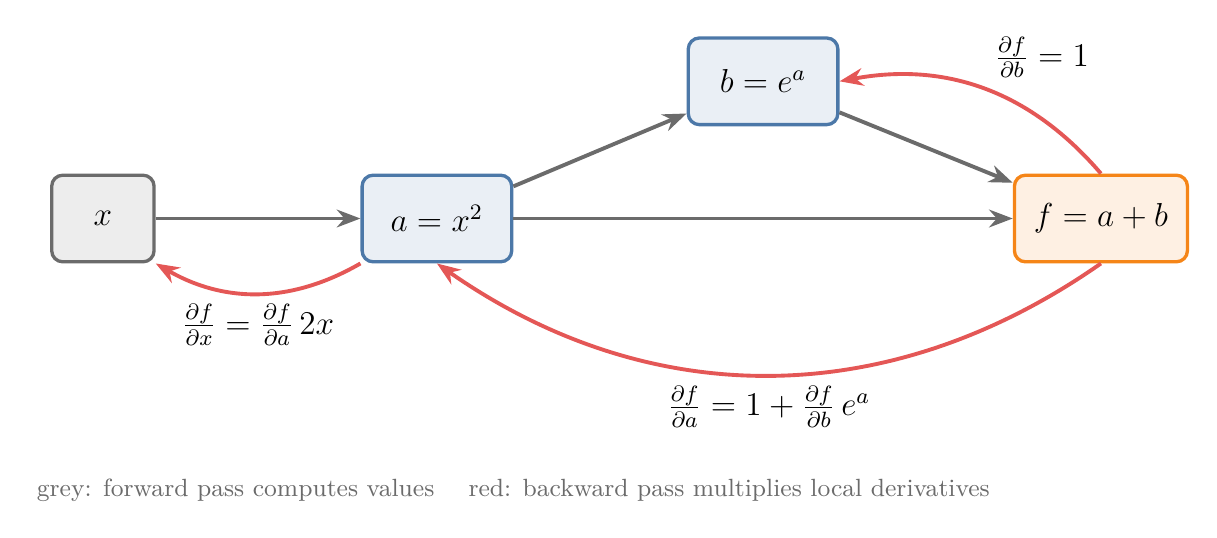
\begin{tikzpicture}[node distance=1.0cm and 2.6cm, every node/.append style={font=\large}]
  \node[box=cgrey, minimum width=1.3cm] (x) {$x$};
  \node[box=cblue, minimum width=1.9cm, right=of x] (a) {$a = x^2$};
  \node[box=cblue, minimum width=1.9cm, above right=0.6cm and 2.2cm of a] (b) {$b = e^{a}$};
  \node[box=corange, minimum width=1.9cm, below right=0.6cm and 2.2cm of b] (f) {$f = a + b$};
  \draw[arrow] (x) -- (a);
  \draw[arrow] (a) -- (b);
  \draw[arrow] (b) -- (f);
  \draw[arrow] (a) -- (f);
  \draw[-{Stealth[length=3mm]}, cred, line width=1.4pt, bend left=35] (f.south) to node[below, font=\large, text=black] {$\frac{\partial f}{\partial a} = 1 + \frac{\partial f}{\partial b}\,e^{a}$} (a.south);
  \draw[-{Stealth[length=3mm]}, cred, line width=1.4pt, bend left=30] (a.south west) to node[below, font=\large, text=black] {$\frac{\partial f}{\partial x} = \frac{\partial f}{\partial a}\,2x$} (x.south east);
  \draw[-{Stealth[length=3mm]}, cred, line width=1.4pt, bend right=30] (f.north) to node[above right, font=\large, text=black] {$\frac{\partial f}{\partial b} = 1$} (b.east);
  \node[note, below=2.6cm of a.south east, anchor=north] {grey: forward pass computes values \quad red: backward pass multiplies local derivatives};
\end{tikzpicture}
\end{document}
